\documentclass{article}

% Language setting
% Replace `english' with e.g. `spanish' to change the document language
\usepackage[english]{babel}

% Set page size and margins
% Replace `letterpaper' with `a4paper' for UK/EU standard size
\usepackage[letterpaper,top=2cm,bottom=2cm,left=3cm,right=3cm,marginparwidth=1.75cm]{geometry}

% Useful packages
\usepackage{amsmath}
\usepackage{graphicx}
\usepackage{appendix}
\usepackage[colorlinks=true, allcolors=blue]{hyperref}
\usepackage{caption}
\captionsetup{justification=centering}

\title{Airframe Analysis}
\author{Ryan Howell}

\begin{document}
\maketitle

%\begin{abstract}

%\end{abstract}

\section{Introduction}

Through reading the textbook and VortexLattice.jl documentation as a part of this assignment, I learned about the Vortex Lattice method. By experimenting with VortexLattice.jl functions, I observed the aerodynamic effects of wing shape, angle of attack, and tail volume ratios. In this report, I will discuss some key takeaways from the reading and will explore the effects of manipulating an airframe and environmental conditions using the panel method. These results will be explained using theory and compared to previous XFoil.jl results.

\section{Background Readings}
The suggested readings covered, in part, the geometry and underlying reason for wing design. It also describes vortices and explains the principles behind the Vortex lattice method. The second chapter of the required reading summarizes the effect of compressible flow at high speeds. 

\subsection{Geometry}
Through the manipulation of sweep, twist, chord, and dihedral angle, you can change the aerodynamics and reference area of the individual wing. However, an unavoidable aerodynamic effect of wing shape is downwash, although it can be limited by expanding the span and selecting wing types such as closed wings. It also changes the effective angle of attack.

\subsection{Vortices}
As the geometry induces downwash and a wake we can map out the vortex filaments created by the wing and simplify the fluid flow. If we assume the trailing vortices go to infinity we get a horseshoe vortex. We can add multiple horseshoe vortices to the wing by sectioning the wing off to add accuracy until eventually, we have a sheet of continuously varying vorticity. 

This is the basis for the vortex lattice method approach. By relating  the lift coefficient to circulation, we can then use this vortex analysis to analyze the aerodynamic properties of an airfoil. This is then extended into three dimensions by creating a lattice structure to find the aerodynamic properties.

\subsection{Compressible Flow}
The importance of compressible flow arises at high speeds. As objects start to travel through fluids at high velocities, the fluid will begin to compress. This compression is limited to the speed of sound through that medium. If you go faster than that speed an instantaneous change in air properties is needed to account for the differences in properties created by compression of the fluid. This causes an instantaneous and sudden change called a shock wave, which for a super sonic airplane is a part of a Mach cone. 

These shock waves bring about new types of drag and considerations in designing planes for high speed travel applications. This then affects the flow properties and behavior of a gas over the wing. This brings about new challenges in characterizing fluid flow over a wing. This can be handled through thin-airfoil theory, inspiring new airfoil shapes. The Mach cone and shock waves likewise influence airplane design.

\section{Effect of Wing Lift Distribution on Efficiency}
The shape of the wing determines many factors such as chord lengths and reference areas. The relationship of these and other variables create different lift coefficients as the shape of the wing changes. I will examine the effect of these wing shapes along with how they effect wing efficiency. These will then be analyzed in the frame of how the vortex lattice approach analyzes these results given different lattice structures. This section presents graphics produced through the properties obtained via the vortex lattice method.

\subsection{Elliptic Wing}
An elliptic wing is a half ellipse for a singular wing or a full ellipse when both wings are put together. To analyze this wing I created a function that creates the wing, leading edge points, and chord lengths given the root chord and span of the wing. A plot of such a wing is shown in Figure \ref{fig:Elliptic wing profile}. 

The first study was of the effect of adding more vertical sections to the wing on the shape and behavior of the lift distribution. As shown in Figure \ref{fig:Elliptic wing lift profile}, as you add sections, the lift distribution seems to approach this flattened elliptic shape. This is true to a point until the increasingly shortened changes and small chord lengths result in a over sensitivity to error and potential spikes in lift as shown.

When comparing the effect of adding sections to the efficiency of the wing, we see that adding sections makes it diverge albeit accurately, from the perfect elliptic curve. This is predicted by the theory for this approach and is shown in Figure \ref{fig:Elliptic Efficiency}. This shows that as we add sections we get a clearer picture of the lift distribution, which is far from the ideal elliptic profile.

\begin{figure}[h]
    \centering
\begin{minipage}[b]{0.45\textwidth}
\centering
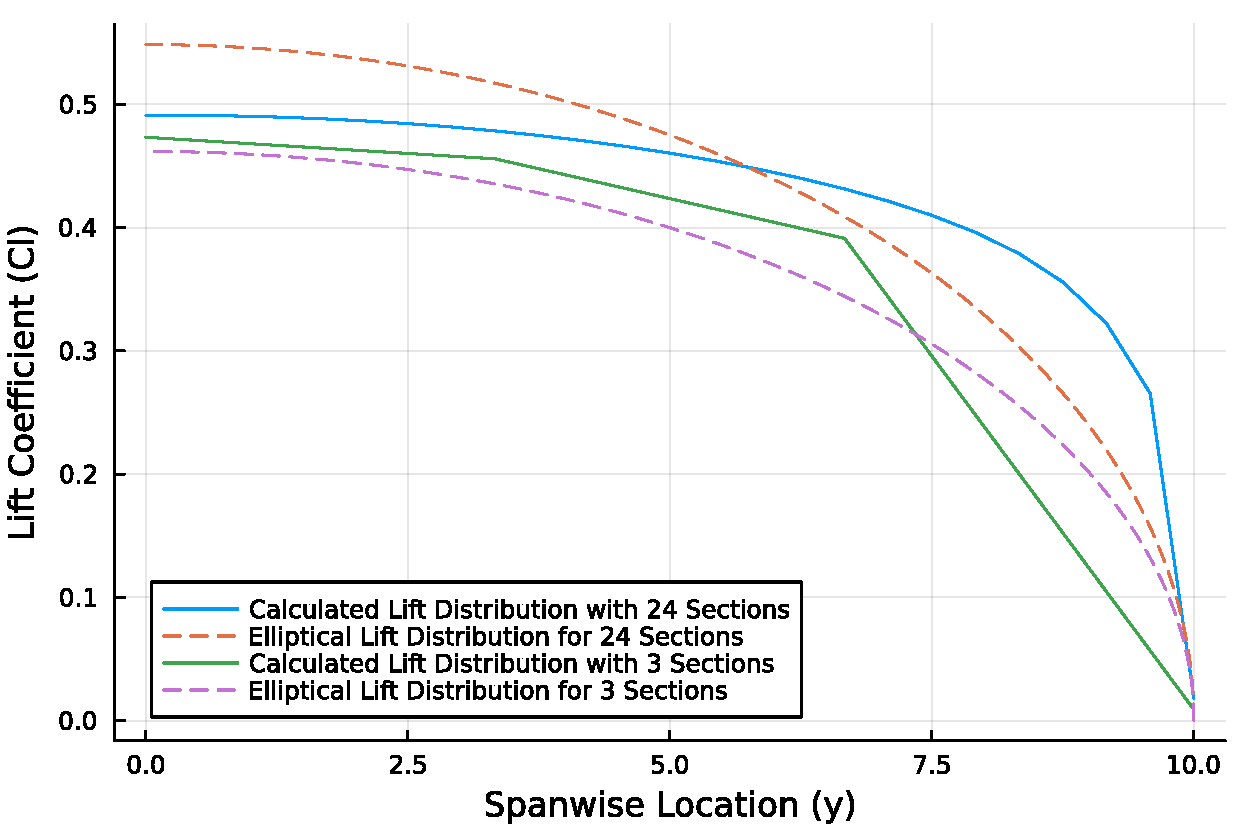
\includegraphics[width=\textwidth]{Lift_Distribution_along_the_Span.pdf}
\caption{Efficiency comparison}
\label{fig:Elliptic Efficiency}
\end{minipage}
\begin{minipage}[b]{0.45\textwidth}
\centering
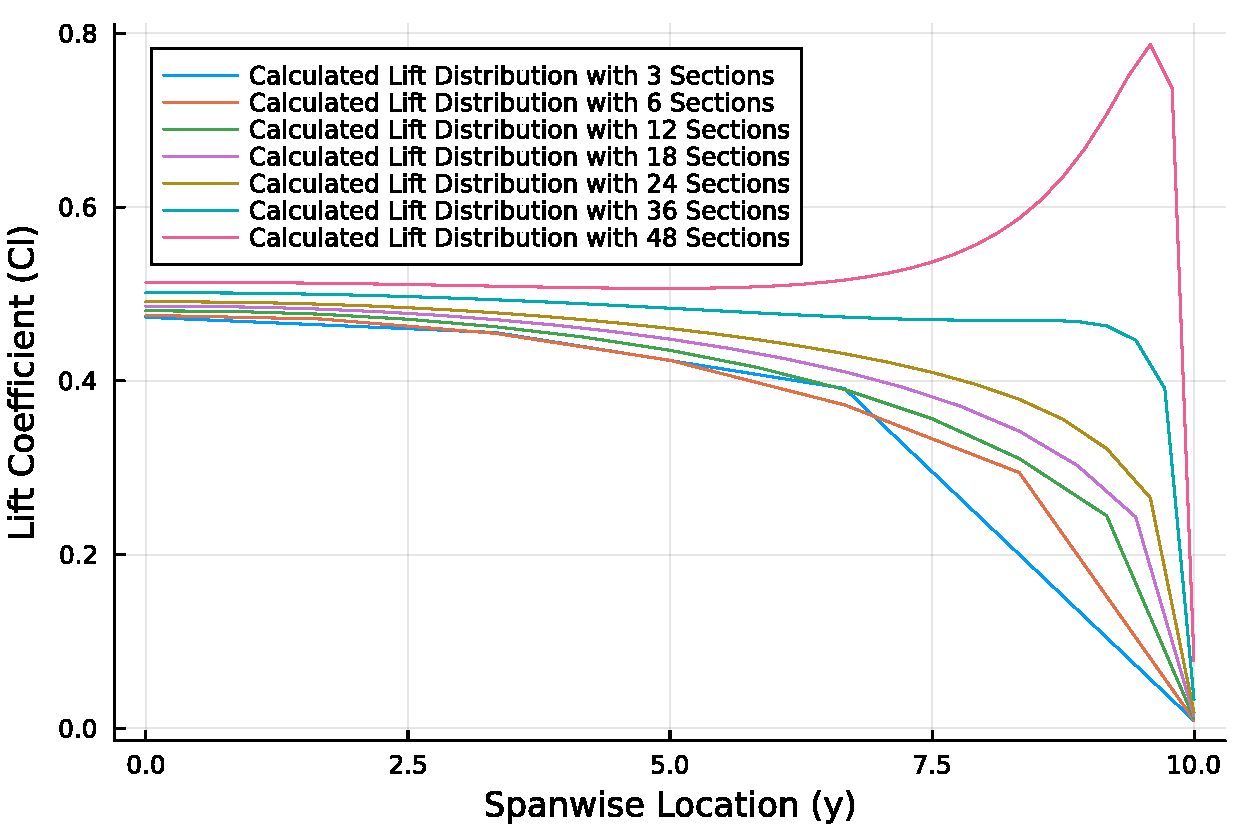
\includegraphics[width=\textwidth]{Lift_Distribution_along_the_Span_Increments.pdf}
\caption{Effect of section size on lift profile}
\label{fig:Elliptic wing lift profile}
\end{minipage}
\end{figure}

\begin{figure}[h]
\centering
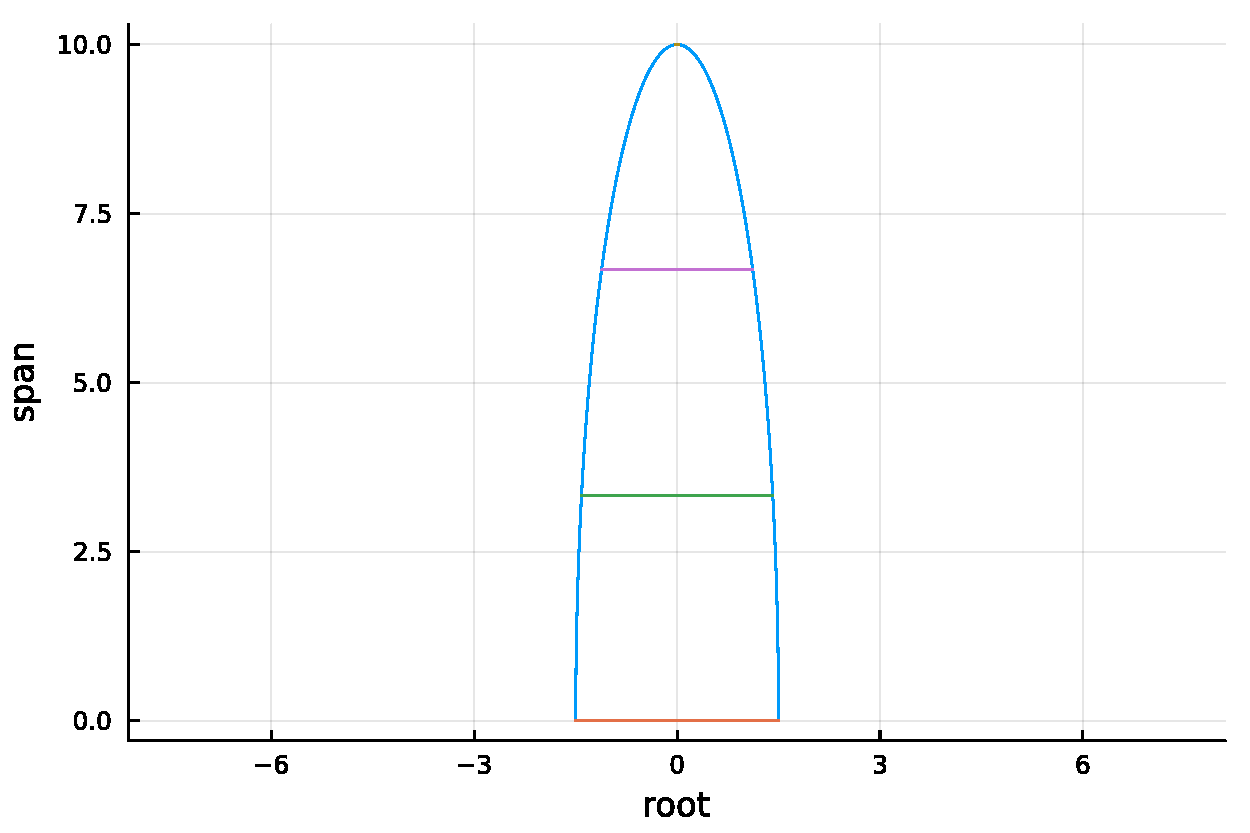
\includegraphics[width=.55\linewidth]{eliptic_wing_section_plot.pdf}
\caption{\label{fig:Elliptic wing profile}An elliptic wing divided in three sections}
\end{figure}

\subsection{Other Wing Shapes}
I also created a function similar to the elliptic wing generator that takes in a tip chord in addition to the previously described variables to produce the necessary information to analyze a quadrilateral wing profile. This allowed me to generate rectangular and tapered wings as shown in Figures \ref{fig:Rect Wing} and \ref{fig:Tap Wing}. 

The lift profiles of these wings also don't align perfectly with an ideal elliptic lift distribution as shown in Figure \ref{fig:Polygonal lift dist}. Yet they are also different. By imagining transitioning between the two we can see that a tapered wing reduces the lift created by the wing, due to less area, but can shift the curve to more closely match the ellipse.

\begin{figure}[h]
    \centering
\begin{minipage}[b]{0.45\textwidth}
\centering
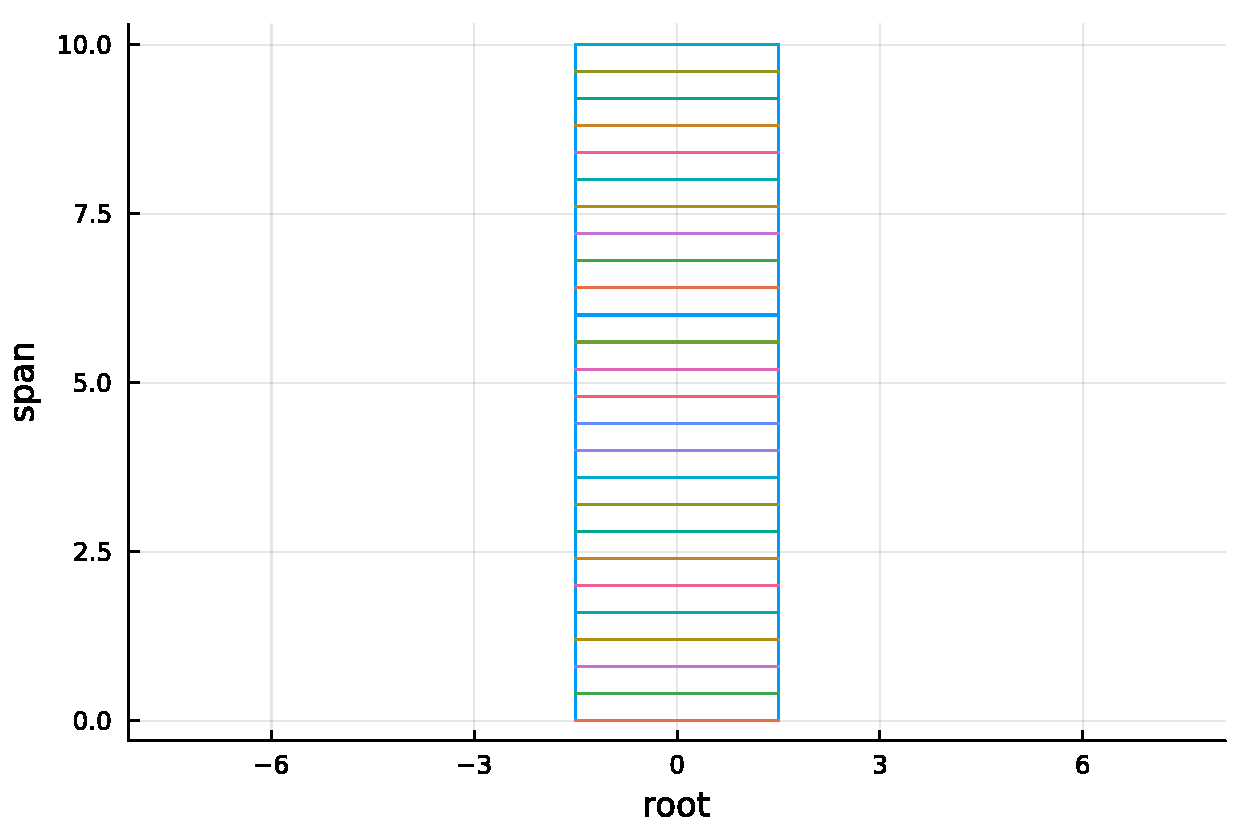
\includegraphics[width=\textwidth]{Rectangular_wing_section_plot.pdf}
\caption{A rectangular wing profile divided into sections}
\label{fig:Rect Wing}
\end{minipage}
\begin{minipage}[b]{0.45\textwidth}
\centering
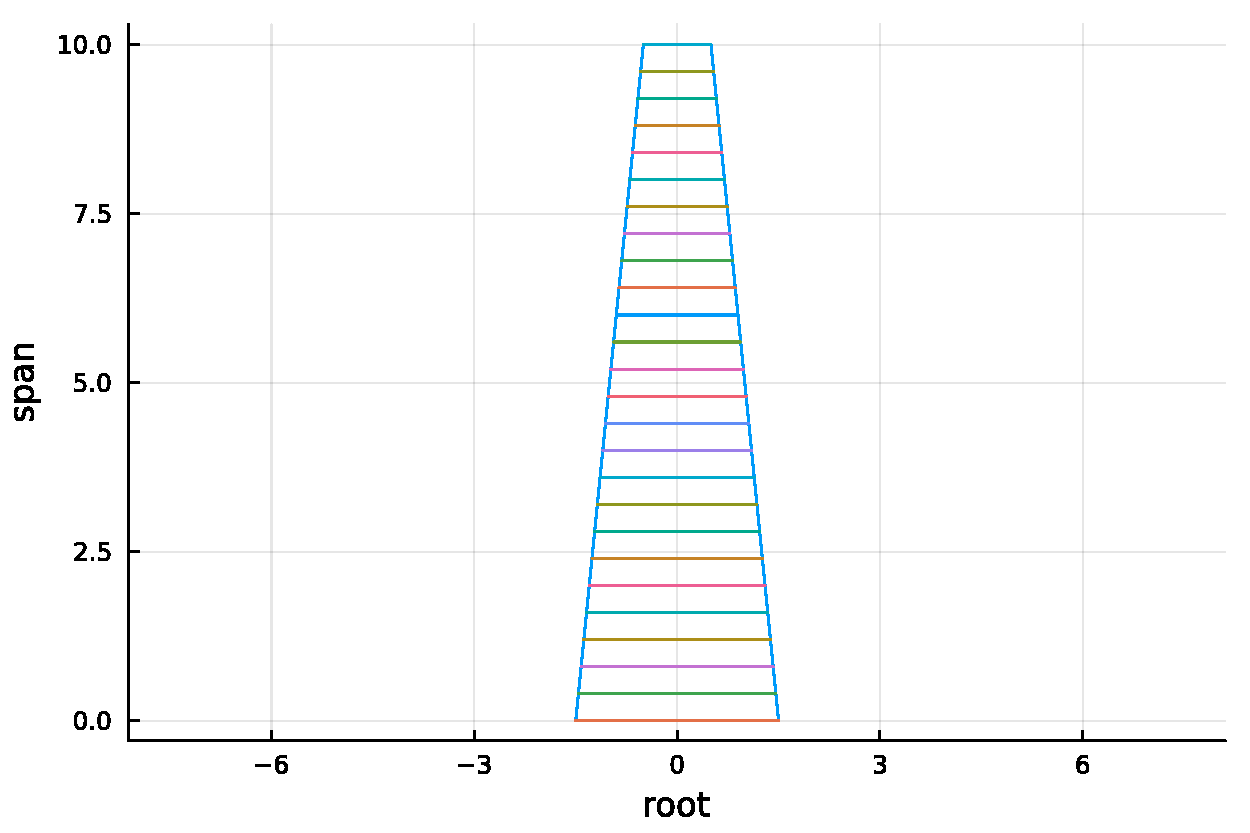
\includegraphics[width=\textwidth]{tapered_wing_section_plot.pdf}
\caption{A tapered wing profile divided into sections}
\label{fig:Tap Wing}
\end{minipage}
\end{figure}

\begin{figure}[h]
\centering
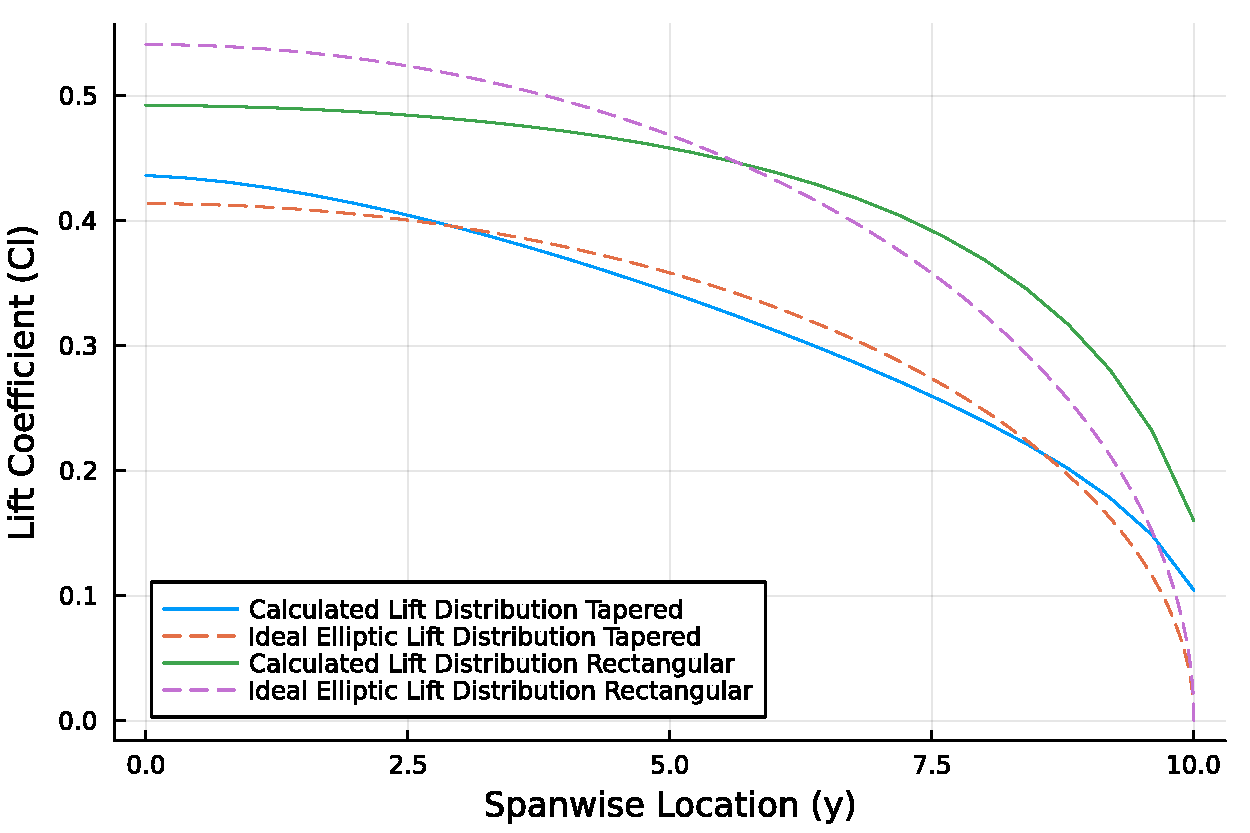
\includegraphics[width=.55\linewidth]{Lift_Distribution_along_the_Span_taper_Iteration.pdf}
\caption{\label{fig:Polygonal lift dist} Polygonal wing shapes lift distributions}
\end{figure}

\section{Tail Volume Ratios and Stability Derivatives}
The tail of a plane through the use of the rudder and elevator, determine the pitch and yaw of a plane. The overall shape of each part of the tail, in turn, affects the stability derivatives of the plane in these directions. A grid of the stability derivatives related to pitch and yaw showing the effect of increasing the horizontal and vertical tail volume ratios is attached as Figure \ref{fig:Complete Chart} in Appendix A. These results, however, include various less interesting results. Figures \ref{fig:Pitch Chart} and \ref{fig:Yaw Chart} focus on the more interesting variable changes caused by changing the horizontal and vertical tail volume ratios respectively.

\subsection{Results}
This larger table in Appendix A shows that the horizontal tail volume ratio has a nearly exclusive effect on the pitch stability-related derivatives. This effect is highlighted in Figure \ref{fig:Pitch Chart}. While the vertical tail volume ratio has a similar effect on the yaw stability-related derivatives, its effect is highlighted in Figure \ref{fig:Yaw Chart}. Examining these charts we see that changing the horizontal tail volume ratio greatly affects the stability derivatives related to angle of attack and pitch rate. Similarly, the vertical tail volume ratio greatly affects the stability derivatives related to the yaw angle and yaw rate.

\begin{figure}[h]
    \centering
\begin{minipage}[b]{0.45\textwidth}
\centering
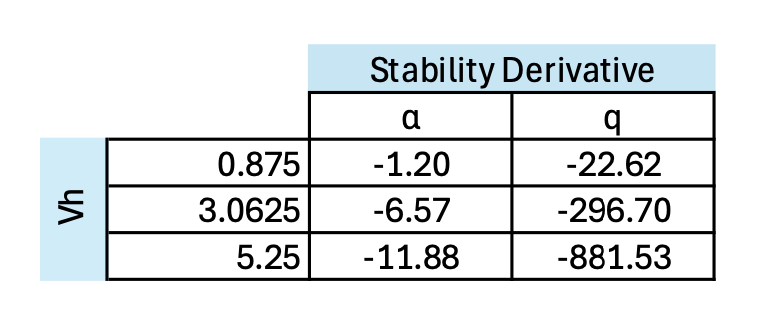
\includegraphics[width=\textwidth]{Pitch Chart.png}
\caption{The effect of solely changing horizontal tail volume on pitch stability derivatives}
\label{fig:Pitch Chart}
\end{minipage}
\begin{minipage}[b]{0.45\textwidth}
\centering
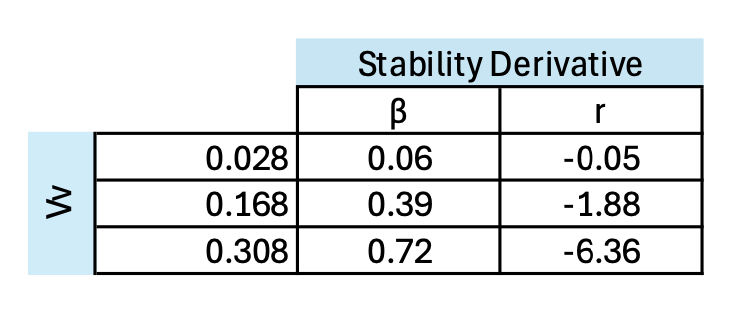
\includegraphics[width=\textwidth]{Yaw Chart.png}
\caption{The effect of solely changing vertical tail volume on yaw stability derivatives}
\label{fig:Yaw Chart}
\end{minipage}
\end{figure}

\section{Effect of Angle of Attack on Lift}

Similar to the lift of an airfoil, the lift of a wing increases with angle of attack, see Figure \ref{fig:lift angle}. 

\subsection{Difference from Xfoil Method}

There are some key differences when compared to the Xfoil.jl plots of airfoils. Firstly, there is no clear stall that occurs as it did in Xfoil.jl shown in my previous report. This is likely due to the lack of viscous effects and subsequently separation, meaning the air is allowed to follow the airfoil closer and not separate. Without separation, there is no wake created that causes stall. This outlines one of the great limitations of the vortex lattice method. 

The limitations of neglecting viscous effects are compounded by the assumption of small angles of attack and sideslip inherent in this method. This means it will maintain a linear shape at high angles, which is an inaccurate assumption. Additionally, the vortex lattice method does not account for compressible flow, thick airfoils, or added complexities in the wake. Despite these limitations, it remains a fairly accurate method for analyzing three-dimensional wings

\begin{figure}[h]
\centering
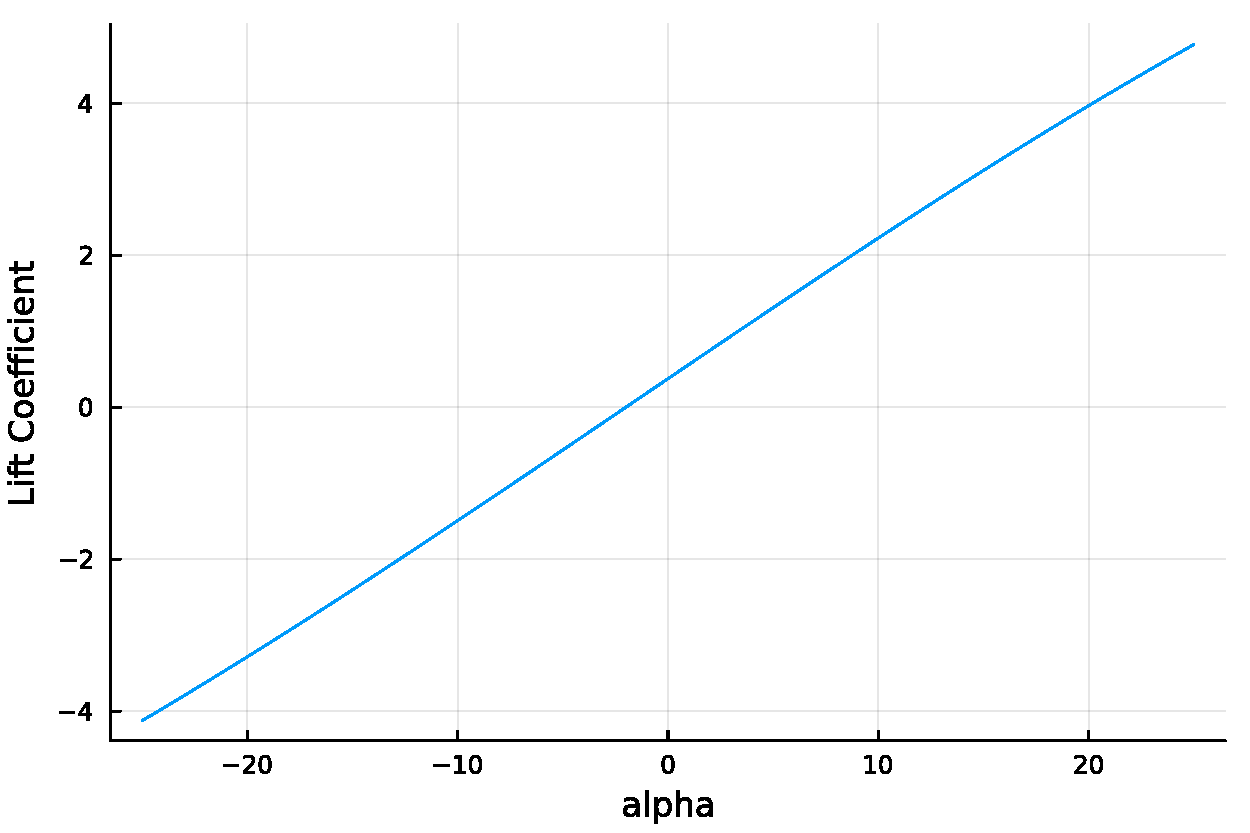
\includegraphics[width=.55\linewidth]{Lift Coefficient vs Angle of Attack.pdf}
\caption{\label{fig:lift angle} Effect of angle of attack on a whole wing}
\end{figure}

%\bibliographystyle{alpha}
%\bibliography{sample}

\clearpage
\appendix
\chapter{Appendix A}

\begin{figure}[h]
\centering
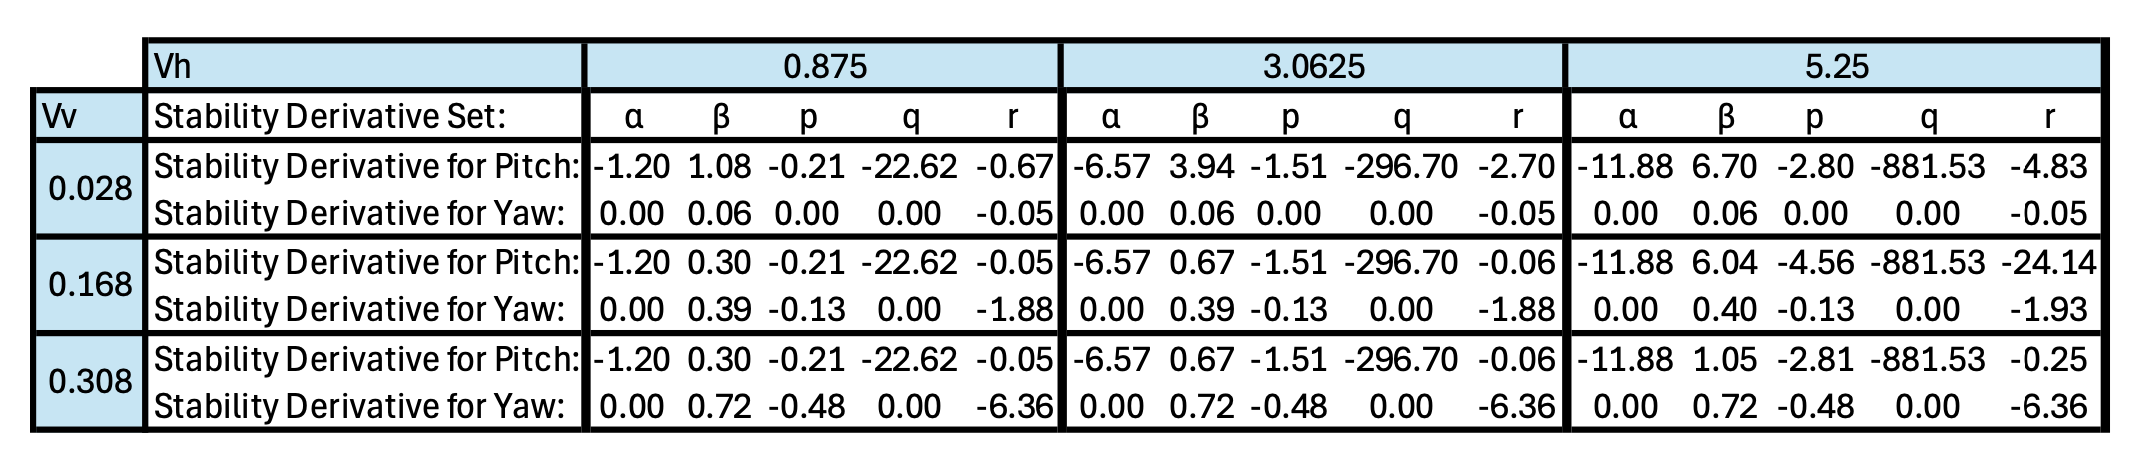
\includegraphics[width=.55\linewidth]{Complete Chart.png}
\caption{\label{fig:Complete Chart} A chart of the effect of horizontal and vertical tail volume ratios}
\end{figure}

\end{document}